\chapter{Bridging the Gap}\label{chapter:solutions}

In the previous chapters, I explored the history of machine learning and provided a comprehensive overview of the most critical aspects of the \ac{MLOps} life cycle, and briefly discussed the reasons for why the gap between running code locally on developer's machine and deploying it in a cloud-based environment for running.
\newline
This chapter aims to introduce strategies for overcoming this gap and its associated challanges. Integrating these strategies requires a comprehensive understanding of both the theoretical and practical aspects of cloud computing and local development environments. It is important to point out that each strategy outlined in this chapter is accompanied by a comprehensive explanation of how it works, and include code examples that demonstrate its practical application.
\section{Containerization}
In order to grasp the concept of containerization, it is essential to understand the concept of vertualization and the differences between various virtualization mechanisms.

\subsection{Virtualization}
Virtualization is the process of creating a virtual version or several virtual versions of a piece of computer or a sofware according to cambridge dictionary \cite{cambridge_dictionary}. It is the art of creating a virtual version of somthing that does not exists physically, appearing as though is does.
\newline
In computer science, virtualization refers to replicating a physical system or server and its components within a single machine, to mimic their functionality. Basically, it is about sharing capabilities of a single physical machine accross multiple users or virtual settings. This approach empowered cloud service providers to share their physical infrastructure capabilities to user more efficiently.

\subsection{Containers vs. Virtual Machines}
We can distinguish between two primary forms of virtualization:
\begin{enumerate}
    \item \textbf{\ac{VMs}}: \ac{VMs} virtualize an entire machine down to the hardware layers. They mimic the behavior of the underlying physical hardware/computer - like CPU, Disks and Networking devices - using a hypervisor, thus creating several virtual machines. Each virtual machine runs its \ac{OS} required for the respective applications, libraries, and functions separately from the other \ac{VMs}. Different \ac{VMs} can be run on the same physical host. Virtual machines may also include a complementary software stack to run on the emulated hardware. These hardware and software packages combined produce a fully functional snapshot of a computational system. As shown in \autoref{fig:Virtual_Machine}
          \begin{figure}[htbp]
    \centering
    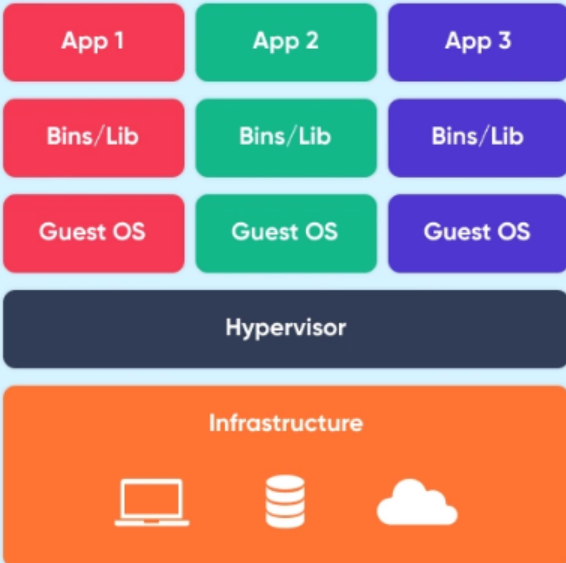
\includegraphics[width=0.4\linewidth]{figures/virtual_machine.png}
    \caption{Structure of vertual machines.}
    \label{fig:Virtual_Machine}
\end{figure}
          \newline
          \textbf{Advantages}
          \begin{itemize}
              \item \textbf{Complete Isolation}: \ac{VMs} operate in total isolation, effectivly wording as independent systems. this isolation ensures that these machine are protected from any harmful exploits, or interference from other \ac{VMs} sharing the same host. While it is still possible for a virtual machine to be vulnerable to some exlpoits, the contaminated virtual machine will not affect the neighboring \ac{VMs} due to this isolation, preventing any cross-contamination amoung virtual machines.
              \item \textbf{Dynamic Development}: \ac{VMs} offer more dynamic development environment. Starting from basic setup, virtual machine can be treated like individual computers. this adaptability enables the direct installation of software, enabling the hands-on development process. Additionally, virtual machines allow for the creating of images, capturing their configurations at any given time.
          \end{itemize}

          \textbf{Disadvantages}
          \begin{itemize}
              \item \textbf{Cost of Storage Space}: It is worth noting that virtual machine take up a lot of space, due to the fact that they virtualize the entire machine. This expansion can lead to potential disk storage issues as the virtual machines keep expanding. Therefor it is crucial to keep monitoring and managing the consumtion to ensure optimal performance and to avoid any disruption on the virtual machine.
              \item \textbf{Speed of Iteration}: Creating and maintaining a virtual machines can be a complex and time-consuming process, as it involves setting up an entire system stack. Modefiying a snapshot of a virtual machine can require significant efforts to rebuild and ensure its expected functionality.  
          \end{itemize}
    \item \textbf{Containers}: Containers take an alternative approach, by bunding the application with its necessary binaries, libraries and dependencies into a single package. Unlike traditional techniques, containers mimic the host operating system, giving each container the illusion of being isolated and that it is interactiting with its own virtual kernal, while the truth is, that all containers on host are sharing the same kernal. As demonstrated in \autoref{fig:Containers}. This shared kernal design alloes one \ac{OS} instance to run several isolated containers, making them lightweight and faster to boot compared to virtual machines. This efficiency is resource management and the accelerated application delivery highlights the advantages of containers over \ac{VMs}.
          \begin{figure}[htbp]
    \centering
    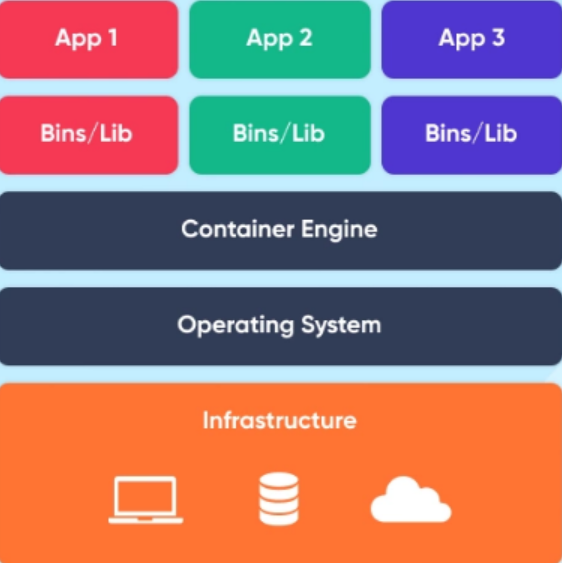
\includegraphics[width=0.445\linewidth]{figures/containers.png}
    \caption{General structure of containers.}
    \label{fig:Containers}
\end{figure}
          \newline
          \textbf{Advantages}
          \begin{itemize}
              \item
          \end{itemize}

          \textbf{Disadvantages}
          \begin{itemize}
              \item
          \end{itemize}
\end{enumerate}
\subsection{Docker}
\subsection{Why Use Docker in Machine Learning}
\subsection{Example}

%% adding a new page to seperate this two sections (for now)
\newpage

\section{Hybrid Approaches}

\section{Cloud Execution}